\documentclass[12pt]{article}
\usepackage{amsmath}
\usepackage{fontspec, xunicode, xltxtra} 
\usepackage{ctex} 
\usepackage{listings}
\usepackage{xcolor}
\usepackage{footmisc}

\lstset{ 
    keywordstyle= \color{blue!70},
    commentstyle= \color{red!50!green!50!blue!50}, 
    frame=shadowbox,
    rulesepcolor= \color{ red!20!green!20!blue!20} ,
    escapeinside=``, 
    xleftmargin=2em,xrightmargin=2em, aboveskip=1em,
    framexleftmargin=2em
} 

\title{NOIP$_{\text{plus}}$模拟赛}
\author{An\_Account}
\date{}
\begin{document}

    \begin{titlepage}
        \maketitle
        \centerline{提前AK的同学请保持安静,不要高声喧哗}
        $\newline\newline\newline\newline\newline$
        \centerline{\begin{tabular}{|c|c|c|c|c|}
            \hline
            题目编号&题目名称&时间限制&内存限制&特殊编译选项\\
            \hline
            1&失落的银之树&1s&256MB&无\\
            \hline
            2&黑根洞穴的宝藏&1s&256MB&-O2\\
            \hline
            3&纳鲁的苹果树&5s&512MB&-O2\\
            \hline
        \end{tabular}}
    \end{titlepage}
    
    \section{T1 失落的银之树}
    silver.in/out/cpp
    \subsection{题目描述}
    为了重启水之元素,奥日来到了银之树下\par
    银之树是一棵有$n$个节点的有根二叉树,奥日需要将银之树的形态转换成一条链的形式,这样才能
    将水之元素的魔力发挥到最大。每次奥日可以选择一个非根节点$u$,然后进行一次左旋或右旋操作\par
    我们这样定义旋转操作\par
    \centerline{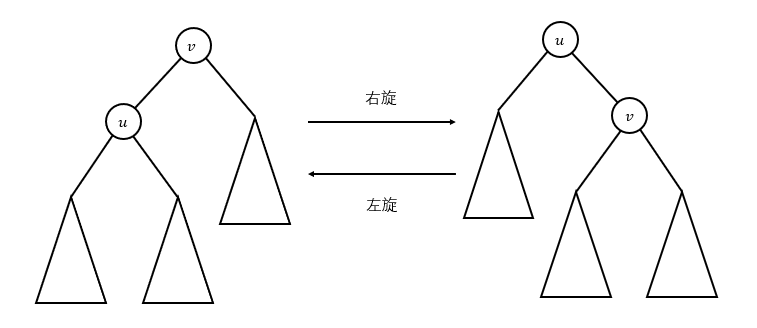
\includegraphics[height=6.0cm, width=12.5cm]{splay.png}}\par
    奥日是一只非常聪明的小精灵,他每次会选择操作次数最少的方案来旋转。
    但是奥日并不知道银之树的具体形态,因此他想知道,对于一种随机的银之树形态,他期望要旋转多少次才能将其变成一条链\par
    注意,\underline{我们认为二叉树的左右儿子是不一样的}
    \subsection{输入格式}
    输入包含两个正整数$n,mod$,分别表示银之树的节点个数以及模数
    \subsection{输出格式}
    输出一个数,表示期望旋转次数模$mod$的余数\par
    假设答案是$\frac{a}{b}$的形式,那么你需要输出正整数$c$使得$cb\equiv a\pmod {mod}$,
    容易证明这样的数在模$mod$意义下只存在一个
    \subsection{样例输入1}
    \lstset{language=C++}
    \begin{lstlisting}
3 1000000007
    \end{lstlisting}
    \subsection{样例输出1}
    \begin{lstlisting}
400000003 
    \end{lstlisting}
    \subsection{样例输入2}
    \begin{lstlisting}
7 1000000007
    \end{lstlisting}
    \subsection{样例输出2}
    \begin{lstlisting}
634032640
    \end{lstlisting}
    \subsection{数据范围}
    对于$30\%$的数据,$n\leq 10$\par
    对于$60\%$的数据,$n\leq 200$\par
    对于$100\%$的数据,$n\leq 500, mod\leq 2*10^9$,保证$mod$是质数
    \subsection{提示}
    对于第一个样例,有如下$5$种情况\par
    \centerline{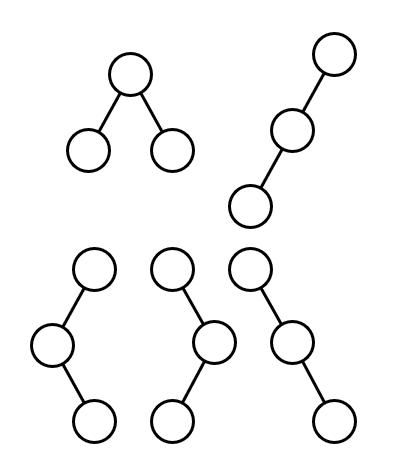
\includegraphics{hint.png}}\par
    其中有且仅有第一种情况需要旋转$1$次,故期望旋转次数为$\frac{1}{5}\equiv400000003\pmod {10^9+7}$\newpage
    \section{T2 黑根洞穴的宝藏}
    cave.in/out/cpp
    \subsection{题目描述}
    They found the home\par
    Of the child who embraced our light\par
    Light and Dark, in innocence born\par
    And though she was lightless\par
    A friendship still formed\par
    But the bond that was made\par
    Would soon be dissolved\par
    After his passing, she left...\par
    And never returned\par
    黑根洞穴中盘亘着精灵之树的树根\par
    树根由大大小小的节点构成,每一个节点都有它对应的能量值。具体来说,第$i$个点有$a_i$的能量\par
    奥日会遍历整棵树,并从中选取一些点吸收对应的精灵之火,第$i$个点的精灵之火为$b_i$\par
    精灵之树是有灵性的,如果节点$u$被奥日选择,那么对于它子树中的节点,奥日只能选取那些能量值\underline{大于等于}$a_u$的点,注意
    精灵之树的根是$1$号节点\par
    你需要帮助奥日求出他最多能收集多少精灵之火\par
    \subsection{输入格式}
    第一行一个整数$n$,表示精灵之树的节点数量\par
    接下来一行$n$个正整数,第$i$个数表示$a_i$\par
    接下来一行$n$个正整数,第$i$个数表示$b_i$\par
    接下来$n-1$行,每行两个整数$a,b$,表示$a,b$之间有一条边
    \subsection{输出格式}
    输出一个数,表示奥日能收集到的精灵之火的最大数量
    \subsection{样例输入}
    \begin{lstlisting}
6
2 4 5 6 3 1
1 7 0 1 2 4
1 2
2 3
2 4
4 5
1 6
    \end{lstlisting}
    \subsection{样例输出}
    \begin{lstlisting}
12
    \end{lstlisting}
    \subsection{数据范围}
    对于前$10\%$的数据,$n\leq 20$\par
    对于前$20\%$的数据,$n,a_i\leq 500$\par
    对于前$30\%$的数据,$n,a_i\leq 2*10^3$\par
    对于另$30\%$的数据,$b_i=1$\par
    对于另$10\%$的数据,第$i$个点与第$i+1$个点相连\par
    对于$100\%$的数据,$1\leq n,a_i\leq 10^5,1\leq b_i\leq 10^9$
    \newpage
    \section{T3 纳鲁的苹果树}
    apple.in/out/cpp
    \subsection{题目描述}
    纳鲁的家后面有一片不大的果园,他想要在里面种一些苹果树\par
    好心的古门送给了他一棵有$n$个点的苹果树,纳鲁把它种了下来\par
    每个苹果都有一个成熟度,一开始所有苹果的成熟度都为$0$\par
    苹果树吸取了精灵之井的能量,每一年,纳鲁都可以选择某一棵苹果树的某个节点$u$,然后将
    这个节点的子树复制一份,种在\underline{这棵苹果树}的右边。注意\underline{苹果的成熟度以及编号也会被同时复制}。\par
    有时,苹果树会慢慢开始成熟,纳鲁会给你一个区间$[l,r]$以及一个编号$u$,表示在当前的第$[l,r]$棵且含有$u$这个节点的所有苹果树中,
    $u$的子树的成熟度$+1$\par
    同时纳鲁还想知道,在某些时刻某一棵苹果树上的某个苹果的成熟度\par
    \subsection{输入格式}
    第一行两个整数$n,q$分别表示最开始的苹果个数以及操作个数\par
    接下来$n-1$行,每行两个整数$a,b$表示第一棵树中$a,b$之间连着一条边\par
    接下来$q$行,每行表示一种操作,具体如下:\par
    \begin{itemize}
        \item $1$ $a$ $b$ 这个操作表示将第$a$棵苹果树中以$b$为根
            的子树复制一份,并编号为第$a+1$棵树。\underline{它后面的苹果树的编号整体$+1$}\par
        \item $2$ $l$ $r$ $u$ 给在$[l,r]$区间中且存在编号为$u$的苹果的树中$u$的子树的成熟度$+1$
        \item $3$ $a$ $b$ 查询第$a$棵苹果树中编号为$b$的苹果的成熟度
    \end{itemize}\par
    \subsection{输出格式}
    对于每个操作$3$输出相应的答案
    \subsection{样例输入}
    \begin{lstlisting}
7 9
1 2
2 4
2 5
2 3
4 6
6 7
2 1 1 7
2 1 1 2
2 1 1 3
1 1 5
2 1 2 6
3 2 5
2 1 2 1
1 1 6
3 2 6
    \end{lstlisting}
    \subsection{样例输出}
    \begin{lstlisting}
1
3
    \end{lstlisting}
    \subsection{数据范围}
    对于$30\%$的数据,$n,q\leq 100$\par
    对于$100\%$的数据,$n,q\leq 10^5$\par
    \subsection{提示}
    一开始只有一棵树\par
    \centerline{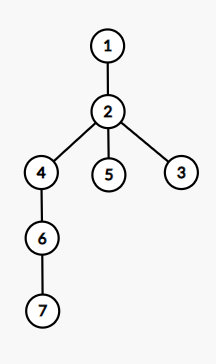
\includegraphics{hint1.png}}\par
    接下来给第一棵树的$7,2,3$号苹果的子树$+1$\par
    \centerline{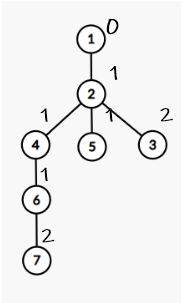
\includegraphics{hint2.png}}\par
    然后复制了$5$号苹果的子树\par
    \centerline{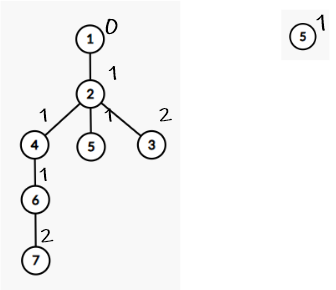
\includegraphics{hint3.png}}\par
    将$[1,2]$中$6$号苹果的子树成熟度$+1$,由于第二棵树没有$6$号节点,因此不管\par
    查询第$2$棵树中$5$号苹果的成熟度,为$1$\par
    接着将$[1,2]$中$1$号苹果的子树成熟度$+1$,由于第二棵树没有$1$号节点,因此不管\par
    \centerline{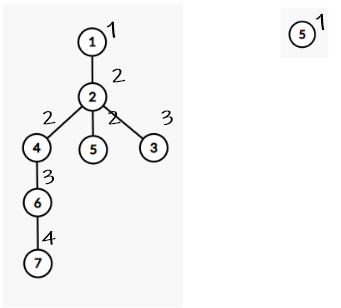
\includegraphics{hint4.png}}\par
    复制第$1$棵树中的$6$号苹果所在的子树\par
    \centerline{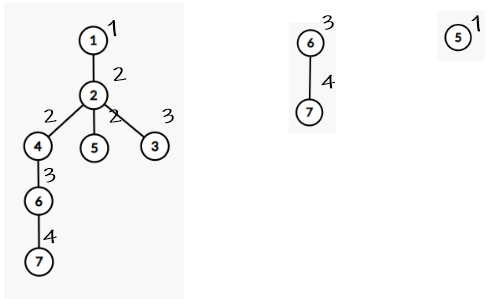
\includegraphics{hint5.png}}\par 
    此时第二棵树中$6$号苹果的成熟度为$3$\par
    \textbf{特别感谢yijian大佬的暴力,以及温爷的强力数据}
\end{document}